\setcounter{chapter}{6}
\chapter{Planar Graphs}
\makeheading{2020-03-23}
$ K_4 $ is the complete graph on $ 4 $ vertices.
There are $ \binom{4}{2}=6 $ edges.

\tikzset{every picture/.style={line width=0.75pt}} %set default line width to 0.75pt        

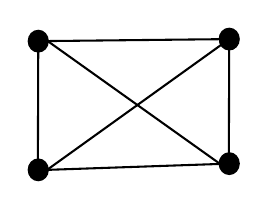
\begin{tikzpicture}[x=0.75pt,y=0.75pt,yscale=-1,xscale=1]
    %uncomment if require: \path (0,310); %set diagram left start at 0, and has height of 310

    %Flowchart: Connector [id:dp40867516170558793] 
    \draw  [fill={rgb, 255:red, 0; green, 0; blue, 0 }  ,fill opacity=1 ] (210,67.8) .. controls (210,65.04) and (212.06,62.8) .. (214.6,62.8) .. controls (217.14,62.8) and (219.2,65.04) .. (219.2,67.8) .. controls (219.2,70.56) and (217.14,72.8) .. (214.6,72.8) .. controls (212.06,72.8) and (210,70.56) .. (210,67.8) -- cycle ;
    %Flowchart: Connector [id:dp9803766535784105] 
    \draw  [fill={rgb, 255:red, 0; green, 0; blue, 0 }  ,fill opacity=1 ] (302,66.8) .. controls (302,64.04) and (304.06,61.8) .. (306.6,61.8) .. controls (309.14,61.8) and (311.2,64.04) .. (311.2,66.8) .. controls (311.2,69.56) and (309.14,71.8) .. (306.6,71.8) .. controls (304.06,71.8) and (302,69.56) .. (302,66.8) -- cycle ;
    %Flowchart: Connector [id:dp012794076729523929] 
    \draw  [fill={rgb, 255:red, 0; green, 0; blue, 0 }  ,fill opacity=1 ] (210,129.8) .. controls (210,127.04) and (212.06,124.8) .. (214.6,124.8) .. controls (217.14,124.8) and (219.2,127.04) .. (219.2,129.8) .. controls (219.2,132.56) and (217.14,134.8) .. (214.6,134.8) .. controls (212.06,134.8) and (210,132.56) .. (210,129.8) -- cycle ;
    %Flowchart: Connector [id:dp26228765510548824] 
    \draw  [fill={rgb, 255:red, 0; green, 0; blue, 0 }  ,fill opacity=1 ] (302,126.8) .. controls (302,124.04) and (304.06,121.8) .. (306.6,121.8) .. controls (309.14,121.8) and (311.2,124.04) .. (311.2,126.8) .. controls (311.2,129.56) and (309.14,131.8) .. (306.6,131.8) .. controls (304.06,131.8) and (302,129.56) .. (302,126.8) -- cycle ;
    %Straight Lines [id:da8965347471664254] 
    \draw    (214.6,67.8) -- (306.6,66.8) ;
    %Straight Lines [id:da2673075983226363] 
    \draw    (219.2,129.8) -- (306.6,126.8) ;
    %Straight Lines [id:da5313322884970586] 
    \draw    (214.6,67.8) -- (214.4,133) ;
    %Straight Lines [id:da004424474413054158] 
    \draw    (306.6,66.8) -- (306.4,132) ;
    %Straight Lines [id:da6155979169107909] 
    \draw    (219.2,67.8) -- (302,126.8) ;
    %Straight Lines [id:da1728251304351116] 
    \draw    (306.6,66.8) -- (214.4,133) ;




\end{tikzpicture}


This picture is not the graph itself, it is a drawing of the graph.
There are other drawings of the same graph.

TODO: K4 planar drawing

`The same graph' means that the vertex set and edge set are the same,
which implies that they have the same set of adjacent pairs.

Informally, a planar drawing of a graph is a way of drawing the graph
in $ \mathbb{R}^2 $ such that the edges do not cross.

TODO: 3-cube non-planar $ V=\{000,001,010,100,110,101,011,111\} $

Clearly, this is a non-planar drawing as there are $ 2 $ crossings
within the graph. However, the $ 3 $-cube can be drawn in a planar way.

TODO: 3-cube planar drawing

\begin{defbox}
    \begin{definition}
        Informally, a \textbf{\emph{planar drawing}} of a graph $ G=(V,E) $
        is a mapping of the vertices of $ G $ to distinct points in
        $ \mathbb{R}^{2} $, and edges of $ G $ to curves between the appropriate
        pair of vertices in such a way that the edges intersect only at their
        common ends.
    \end{definition}
\end{defbox}

\begin{defbox}
    \begin{definition}
        A graph is \textbf{\emph{planar}} if it has a planar drawing.
    \end{definition}
\end{defbox}

\begin{exbox}
    \begin{example}[Planar]
        $ K_4 $ and the $ 3 $-cube are both planar graphs.
        \begin{remark}
            It is \textbf{not} correct to say that $ K_4 $ is \emph{sometimes}
            planar depending on how you draw it. It \textbf{is} correct to say
            that $ K_4 $ is a planar graph because there exists a planar drawing.
        \end{remark}
    \end{example}
\end{exbox}

This definition is quite hard to work with to show a graph is
\emph{not planar}. In fact, there is no obvious way
to prove there \emph{exists} a graph that is not planar since there exists
`infinitely' many possible ways to draw a graph.

TODO: $ K_5 $

has five crossings.

TODO: $ K_5 $

has one crossing.

Clearly, it is hard to see whether $ K_5 $ is planar/non-planar.

Notice that whether you have a planar drawing, you have \emph{faces}.

TODO: graph 7 vertices here

5 faces

TODO: another planar graph

3 faces

\begin{remark}
    Many definitions about graph theory within this course will be informal,
    as defining them with rigour will be time consuming. Formal definitions
    can be found in a course like CO 342 (Introduction to Graph Theory),
    and courses about Topology.
\end{remark}

\begin{defbox}
    \begin{definition}
        Given a drawing of a graph,
        let $ X $ be the set of points of $ \mathbb{R}^2 $ that
        are part of the drawing. Informally, the \textbf{\emph{faces}}
        of the drawing are the `connected regions'
        of $ \mathbb{R}^2\setminus X $.
    \end{definition}
\end{defbox}

\begin{remark}
    A planar drawing of a graph is also called an \textbf{\emph{embedding}}.
\end{remark}

TODO: planar graph (20 min)

Each face of a connected planar drawing has a boundary walk. This is a
closed walk of the graph that follows the boundary of the
face.

The boundary walk for $ f_2 $ is:
\[ (v_3,e_3,v_4,e_4,v_5,e_5,v_6,e_6,v_7,e_7,v_3) \]

If an edge $ e $ belongs to the boundary walk, of a face $ f $,
we say that $ e $ is \textbf{\emph{incident}} with $ f $.

If two faces have boundary walks that share an edge,
then they are \textbf{\emph{adjacent}}.

The \textbf{\emph{degree}} of a face is the length of its
boundary walk (the number of edges in the walk counting repetitions
twice). $ f_1 $ has degree $ 3 $,
$ f_2 $ has degree $ 6 $, and $ f_3 $ has degree $ 9 $.

\textbf{Q}: Do the edges in a planar drawing need to be straight
lines?

\textbf{A}: No. (THEOREM (Fary $ \approx 1950 $). It doesn't matter).

TODO: 35 min

\textbf{Q}: What about other surfaces than the plane?

\textbf{A}:
\begin{itemize}
    \item $ \mathbb{R}^3 $? Too easy.
    \item Sphere? Interesting.
    \item Torus?
\end{itemize}

\begin{thmbox}
    \begin{prop}
        The graphs that can be drawn on a sphere (without crossings)
        are just the planar graphs. That is, $ G $ can be drawn
        on a sphere (without crossings)
        if and only if $ G $ can be drawn on the plane.
    \end{prop}
\end{thmbox}

Sketch of \emph{proof}:

$ (\impliedby) $ Obviously true. Planar drawing implies spherical drawing.

$ (\implies) $ Take a hole of a balloon, and stretch it (provided the balloon
does not burst). Eventually, it will end up as a flat surface.

\section{Stereographic Projection}
Think about a sphere on a flat surface. Shine the light source onto the sphere
and a shadow will be casted onto the flat surface.

A 'light source' at $ (0,0,1) $ casts a 'shadow' of the graph on the sphere as
a graph on the plane.

\textbf{Q}: Which graphs can we draw on the torus?

\textbf{A}:
\begin{itemize}
    \item $ K_5 $ is an example of a graph that can be drawn on
          a torus, but cannot be drawn on a plane.
    \item $ K_6 $?
    \item $ K_7 $?
\end{itemize}
